\chapter{dHvA measurements on \BaFeP}

This chapter presents a close to definitive measurement of the Fermiology of \BaFeP and also presents extensive data and analysis in to the thermal and spin effective masses. Nesting conditions along the $(\pi,\pi)$ vector where investigated through calculations based on insight gained from the measurements  and partial nesting was found along $q=(\pi,\pi,k_z)$ where $k_z=0,\pi/2,\pi,3\pi/2,2\pi$. Given \BaFeP is not superconducting this suggests that partial nesting is not a sufficient condition for superconductivity.


\section{X-Ray Diffraction}
    \label{Sec:ResD:XrayDiffraction}

The crystalline axes of the sample were determined by \ac{XRD} on a Kappa Apex II single crystal diffractometer with the aid of Dr. M. Haddow. The sample was mounted on a glass rod and held in place using vacuum grease. Clear diffraction spots are visible on the example scans shown in figure~\ref{Fig:ResD:XRayDiffraction} although there is some evidence of a second, misaligned phase with the doubling of the spots in a small number of the scans such as the one in the top left panel. There is also further evidence of secondary phases as some peaks are doubled up in the dHvA data presented later. We have no reason to believe however that these speculated misalignments are significantly affecting the rest of the body of results nor that they affect the conclusions in any appreciable way.

Perhaps surprisingly, the straight edge of the crystal was found to lie along the $[110]$ direction and not along the unit cell axis. This was found to be the case for a number of other \BaFeAsP{} crystals which were x-rayed later in the year.

\begin{figure}[htbp]
    \begin{center}
        \includegraphics[scale=0.7]{Chapter-dHvABaFe2P2/Figures/Xrays/XRayDiffraction/XRayDiffraction}
        \caption{Panels show example diffraction patterns of the \BaFeP{} sample. Left shows a zoomed portion of doubled peaks indicating that there may potentially be a misalignment within the crystal. Right inset shows the labelled crystal axes superimposed on the sample which is mounted on a glass rod.}
        \label{Fig:ResD:XRayDiffraction}
    \end{center}
\end{figure}

Lattice parameters are determined using the Apex II software and are presented in table~\ref{Table:ResD:LatticeParams} along with comparisons to two previous measurements found in the literature. The result agree within the error.
\begin{table}[htbp]
    \begin{center}
        \caption{Lattice parameters from \ac{XRD} measurements compared with literature.}
        \begin{tabular}{llll}
\toprule
Source  &  $a$ (\AA) & $c$ (\AA) & $z_P$ (\% $c$)\\
\midrule
X-ray   & $3.86(4)$  & $12.42(9)$ & \\
Rotter \etal~\cite{Rotter2010} & $3.8435(4) $ & $12.422(2)$ & $34.59(1)$ \\
Mewis \etal~\cite{Mewis1980} & $3.8400$ & $12.4420$ & $34.560$ \\
% Mewis \etal~\cite{Mewis1980} & $3.63$ & $11.76$ & $34.56$ \\
\bottomrule
        \label{Table:ResD:LatticeParams}
        \end{tabular}
    \end{center}
\end{table}



\section{Angle dependent measurements}
    \label{Sec:ResD:AngleDependentMeasurements}

\subsection{Determining experimental parameters}

Preliminary measurements showed very strong \ac{dHvA} oscillations which begin at relatively low field with an example of the raw data shown in figure~\ref{Fig:ResD:RawOscillations}. Since it is not clear from the raw torque data where the oscillations begin, Fourier transforms were taken with small (\unit{1}{\tesla}) field intervals --- the interval where a clear signal is present marks the onset of oscillations. An \ac{FFT} of the data for the ranges \unit{4-5}{\tesla}, \unit{5-6}{\tesla} and \unit{6-7}{\tesla} are shown in the insets of the figure. The range \unit{6-7}{\tesla} clearly shows the electron peaks at around \unit{1500}{\tesla} and \unit{2450}{\tesla}, with the higher frequency peak disappearing in the \unit{5-6}{\tesla} range and both peaks disappearing in the \unit{4-5}{\tesla} range. Further refinement suggests the onset of appreciable oscillations is around \unit{5.6}{\tesla} for the strongest electron peak. The field was ramped between \unit{6}{\tesla} and the safe maximum of \unit{18}{\tesla} for the vast majority of measurements bar some sweeps where the magnet was ramped to or from \unit{0}{\tesla} following or preceding shut-down of the magnet.

\begin{figure}[htbp]
    \begin{center}
        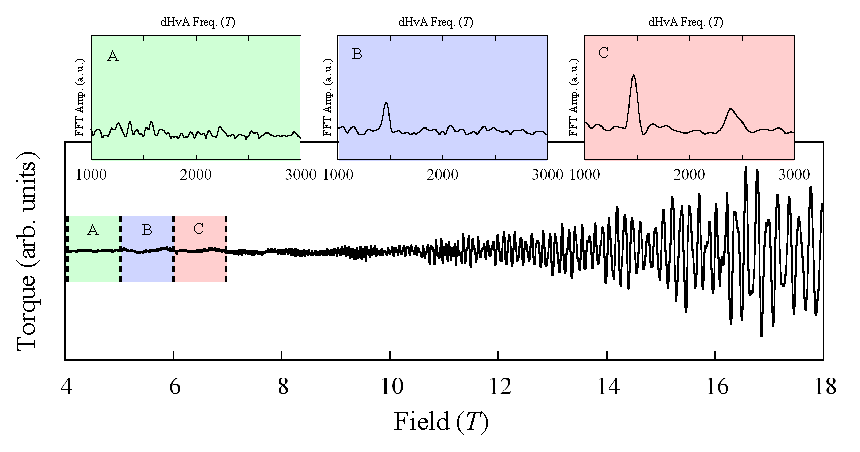
\includegraphics[scale=0.7]{Chapter-dHvABaFe2P2/Figures/AngleDepMeasurements/RawOscillations/RawOscillations}
        \caption{An example of the torque data taken with field aligned at \unit{26}{\degree} on the reverse side of the $[001]$ to $[100]$ angle sweep detailed later. Insets show a \acp{FFT} of the data between \unit{4-5}{\tesla}, \unit{5-6}{\tesla} and \unit{6-7}{\tesla} respectively. These intervals are marked on the main plot as A, B and C.}
        \label{Fig:ResD:RawOscillations}
    \end{center}
\end{figure}

Figure~\ref{Fig:ResD:ComparisonSweepRates} shows some example Fourier transforms of data taken at various field sweep rates and plotted with the frequencies shifted arbitrarily for ease of comparison. The difference in amplitude between the sweeps at \unit{0.05}{\tesla\reciprocal\minute} and \unit{0.1}{\tesla\reciprocal\minute} is less than \unit{1}{\%} whereas the difference when sweeping at \unit{0.2}{\tesla\reciprocal\minute} is nearly \unit{5}{\%}. Unless otherwise stated, subsequent sweeps were performed at \unit{0.15}{\tesla\reciprocal\minute} at the edge of where the sweep rate makes a significant difference in amplitude.

\begin{figure}[htbp]
    \begin{center}
        \includegraphics[scale=0.7]{Chapter-dHvABaFe2P2/Figures/AngleDepMeasurements/SweepRateComparison/SweepRateComparison}
        \caption{FFTs showing the peak from the smaller branch of band $3$ taken at, A: \unit{0.05}{\tesla\reciprocal\minute}, B: \unit{0.1}{\tesla\reciprocal\minute} and C: \unit{0.2}{\tesla\reciprocal\minute}. The peaks are arbitrarily shifted in frequency for ease of comparison. Measurements taken with $H$ at \unit{10}{\degree} from $[001]$ in the $[110]$ direction.}
        \label{Fig:ResD:ComparisonSweepRates}
    \end{center}
\end{figure}

In order to make a reasonable determination of the Fermi surface of a material, an appropriate number of angle sweeps need to be made to adequately constrain the shape of the Fermi surface. Since \BaFeP is a tetragonal system, any sweep from the azimuthal direction $[001]$ down the polar plane effectively expands to four due to the fourfold symmetry. Measurements were taken at one degree intervals from $H\parallel[001]$ down to $H\parallel[100]$ and from $H\parallel[001]$ down to $H\parallel[110]$ which, in this system, effectively amount to eight sweeps.

\begin{figure}[htbp]
    \begin{center}
        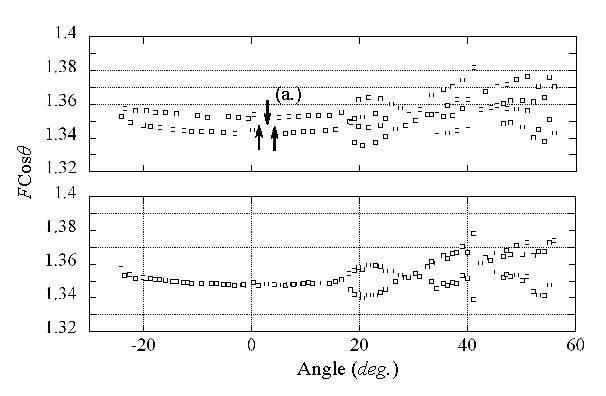
\includegraphics[scale=0.9]{Chapter-dHvABaFe2P2/Figures/AngleDepMeasurements/HysteresisCorrection/HysteresisCorrection}
        \caption{The plots show the $F\cos \theta$ for the $\alpha$ branch in the $[100]$ direction. Top panel shows the branch with the hysteresis due to field sweep direction, the bottom panel shows the data after the linear adjustment described in the main text. Arrows at point (a.) show how the points were shifted.}
        \label{Fig:ResD:HysteresisCorrection}
    \end{center}
\end{figure}

In general, runs were performed with an excitation voltage of \unit{1}{\volt}. To ensure that there was no self heating effects, runs were also performed with an excitations voltage of \unit{0.5}{\volt} and \unit{2}{\volt} at $T\approx$\unit{0.6}{\kelvin} (where we expect the \ac{LK} curve to be steep) and no change in oscillation amplitude due to heating was observed.

The magnetic field was alternatively ramped up and then down meaning subsequent measurements were generally performed with the magnetic field ramping in opposite directions. Although in theory this should not affect the results in any way, subsequent \ac{FFT} peaks appeared to alternately be shifted by up to $\sim\pm$\unit{21}{\tesla} with the magnitude of the shifts being roughly proportional to frequency. Assuming that the shifts were an artefact of the measurements, a linear correction determined by visual inspection was applied of $F_{\textrm{corr.}} = 3 + \frac{10}{8000} F_{\textrm{meas.}}$ for the sweep in the $[100]$ direction and $F_{\textrm{corr.}} = 0 + \frac{21}{8000}  F_{\textrm{meas.}}$ and  $F_{\textrm{corr.}} = 0 + \frac{18}{8000} F_{\textrm{meas.}}$ for the two sets of measurements performed to complete the sweep in the $[110]$ direction. Figure~\ref{Fig:ResD:HysteresisCorrection} shows an example of these hysteric shifts and the subsequent correction applied.

\begin{figure}[htbp]
    \begin{center}
        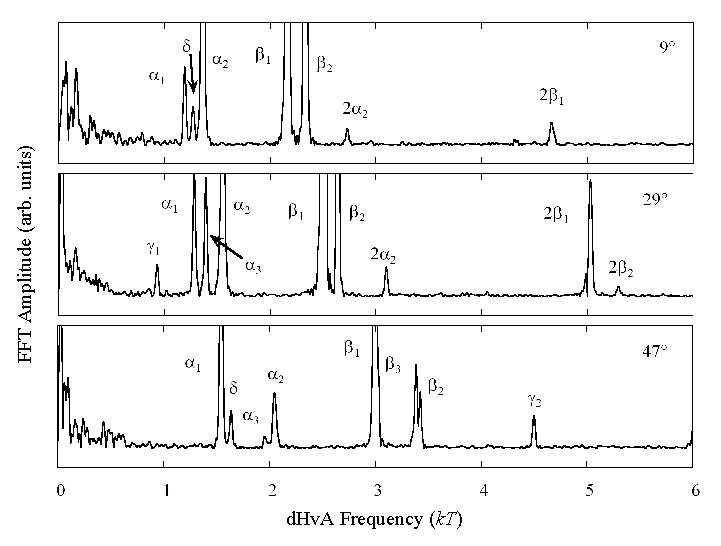
\includegraphics[scale=0.7]{Chapter-dHvABaFe2P2/Figures/AngleDepMeasurements/FFTExamples/FFTExamples}
        \caption{\ac{FFT} after a second order polynomial background was subtracted at various labelled angles between $[001]$ and $[110]$. The labels for peak identification are explained in the next section.}
        \label{Fig:ResD:FFTExamples}
    \end{center}
\end{figure}

Figure~\ref{Fig:ResD:FFTExamples} shows three example \acp{FFT} which show peaks from all the principal bands identified the next section. They also show first and second harmonics\footnote{Third harmonics were also identified in other \acp{FFT}, these are shown in figure~\ref{Fig:ResD:AngleSweepMeasured}.}. The low frequency region in figure~\ref{Fig:ResD:FFTExamples} shows noise from the cantilever, but according to \ac{DFT} fits performed in the next section, this region also likely contains signal from the minimum of band $1$. Given that the signal from electron bands is generally small due to high scattering rate, we were not able to extract a convincing Fourier peak.

Figure~\ref{Fig:ResD:AngleSweepMeasured} shows the \ac{FFT} frequency of peak data multiplied by $\cos\theta$ after having the angle determined as described in section~\ref{Sec:2:AngleCorrection}.  Signal can be observed up to relatively high angles with peak observed almost up to $80\degree$ in the $[110]$ direction which, along with the observation of third harmonics, and the onset of oscillations in relatively low field is testament to the high quality of the crystal.

\begin{figure}[htbp]
    \begin{center}
        \includegraphics[scale=0.9]{Chapter-dHvABaFe2P2/Figures/AngleDepMeasurements/AngleSweepMeasured/AngleSweepMeasured}
        \caption{Peaks identified by varying the field range, window type and background polynomial. Left panel shows data taken with the field parallel to $[001]$ down to $[110]$, the right panels shows $[001]$ to $[100]$.}
        \label{Fig:ResD:AngleSweepMeasured}
    \end{center}
\end{figure}

The left panel in figure~\ref{Fig:ResD:IdentifyingBands} shows the measured rotation data (circles) for the plots towards the $[100]$ direction and in addition the data from the $x=0.63$ data in the \BaFePAs series multiplied by amounts commensurate to the expected shifts in the Shishido paper\cite{Shishido2010} (black squares). We can see that while the size of the areas changes between the two values, the overall shape of the $x=0.63$ data matches reasonably well with the data for $x=1$ for bands 2, 3 and 4 at least. Assuming that nothing exotic happens in the intermediary, we can extrapolate the shape of these Fermi surfaces across the range by applying the known electron Fermi surface areas and the compensation condition. This is explored further in the next section.

\begin{figure}[htbp]
    \begin{center}
        \includegraphics[scale=1.0]{Chapter-dHvABaFe2P2/Figures/AngleDepMeasurements/IdentifyingBands/IdentifyingBands}
        \caption{Left panel shows the measured data with points overlayed from BaFe$_2$(As$_{0.37}$P$_{0.63}$)$_2$\cite{Analytis2010c} with the $\alpha$ and $\gamma$ frequencies multiplied by $1.33$ and $\beta$ frequencies multiplied by $1.19$ commensurate with known shifts from literature. Right panel shows \ac{DFT} calculations (lines) overlayed on top of measured \ac{FFT} data (circles). Data is color coded according to the corresponding bands. Points in grey are harmonics.}
        \label{Fig:ResD:IdentifyingBands}
    \end{center}
\end{figure}



\subsubsection{Rigidly shifting the calculated \ac{DFT} energies}
    \label{Sec:ResD:DFTShifts}

The right panel of figure~\ref{Fig:ResD:IdentifyingBands} shows the \ac{DFT} calculations performed using the augmented plane wave method plus local orbits method method as implemented in the WIEN2k package\cite{Blaha2001}. The unit cell used was that measured by Mewis et al. which are listed in table~\ref{Tab:ResD:LatticeParams} and the subsequent \ac{DFT} calculations were processed into rotation plots using MATLAB code originally written by Dr. Ed Yelland. Results are shown superimposed over the measured data. By factoring the frequency with $\cos{\theta}$ it becomes clearer which of the orbits is a maximal extrema and which is a minimal extrema. Using this knowledge as well as clues from the Fourier amplitude of the measured data, it was possible to separate out individual bands which have been colour coded and labelled --- according to literature convention --- as specified in table~\ref{Tab:ResD:BandNaming}. Minimal extrema are sub-labelled $1$, maxima are sub-labelled $2$. The points marked in grey are the harmonics which were identified by overlaying the measured data on itself after doubling and tripling of the frequency.

\begin{table}
    \begin{center}
        \caption{A summary of the Fermi surface labelling used.}
        \begin{tabular}[htbp]{llll}
\toprule
Band Num.  & Label & Colour    & Type \\
\midrule
1   & $\delta$  & Orange    & hole \\
2   & $\gamma$  & Red   & hole \\
3   & $\beta$   & Blue  & electron \\
4   & $\alpha$  & Green & electron \\
\bottomrule
        \label{Tab:ResD:BandNaming}
        \end{tabular}
    \end{center}
\end{table}

As with previous \ac{DFT} calculations in the \BaFePAs series, the calculated values are consistently higher than the measured values\cite{Shishido2010}. The exception in this case is $\gamma_2$ which is not much different from the calculated values.

As is shown in figure~\ref{Fig:ResD:AngleSweepMeasuredUnshifted}, the rotation plots from the \ac{DFT} calculations match up qualitatively with the data but do not match up quantitatively -- the electron bands overestimating the size of the measured extremal orbits. 

\begin{figure}[htbp]
    \begin{center}
        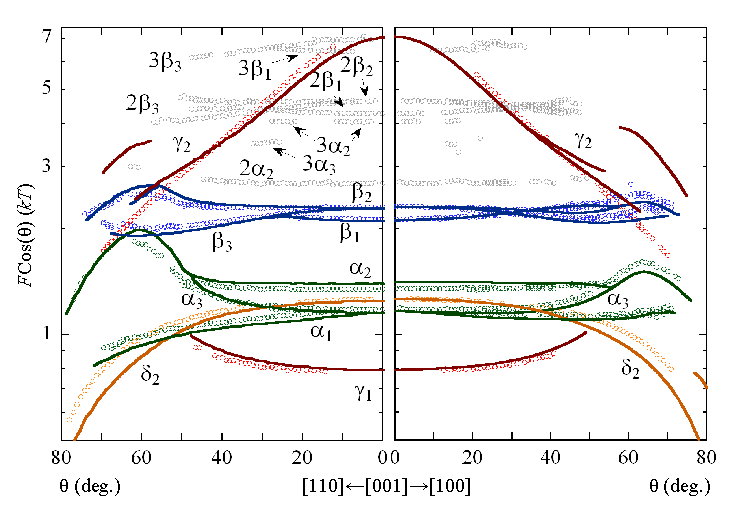
\includegraphics[scale=0.9]{Chapter-dHvABaFe2P2/Figures/AngleDepMeasurements/AngleSweepRigidShift/AngleSweepRigidShift}
        \caption{\ac{dHvA} frequencies multiplied by $\cos(\theta)$. Solid lines are rigidly shifted \ac{DFT} calculations, open circles are measured data. $H$ field directed along $[001]$ towards (a.) $[001]\rightarrow[100]$ and (b.) $[001]\rightarrow[110]$.}
        \label{Fig:ResD:AngleSweepRigidShift}
    \end{center}
\end{figure}

In order to obtain the correct shape of Fermi surface, the \ac{DFT} calculations need to be tweaked. One technique is to apply small band-specific rigid energy shifts, which, in most cases is enough to bring the \ac{DFT} in line with the experimental data. Figure~\ref{Fig:ResD:AngleSweepRigidShift} shows the rotation plots which rotate towards both the 100 and 110 directions along with appropriately shifted calculations. Table~\ref{Tab:ResD:EnergyShifts} lists those energy shifts.
\begin{table}
    \begin{center}
        \caption{Rigid energy shifts required to match the \ac{DFT} calculations with the measured data.}
        \begin{tabular}[htbp]{llr}
\toprule
Band    & \multicolumn{2}{l}{Energy Shift (Ry)} \\
\midrule
1       &       & -0.0083      \\
2       & Wide  & 0.0          \\
        & Narrow & -0.0038     \\
3       &       & 0.0043       \\
4       &       & 0.0050        \\
\bottomrule
        \label{Tab:ResD:EnergyShifts}
        \end{tabular}
    \end{center}
\end{table}

Band $2$ in this case has two separate shifts specified in two different regions of the \ac{BZ}. The rotation plot for the wider orbit located at the edge of the \ac{BZ} was calculated with no energy shift and the narrow part of the Fermi surface around the $\Gamma$ point was calculated with a shift of $\unit{0.0038}{Ry}$. This provides a reasonable match for the rotation plot where we can apply the shift to the two regions discretely, however is proves problematic when we wish to study intermediate areas since it is not clear how the Fermi surface varies between the two regions. A technique for applying appropriate energy shifts throughout the \ac{BZ} is explored in the next section.

\begin{figure}[htbp]
    \begin{center}
        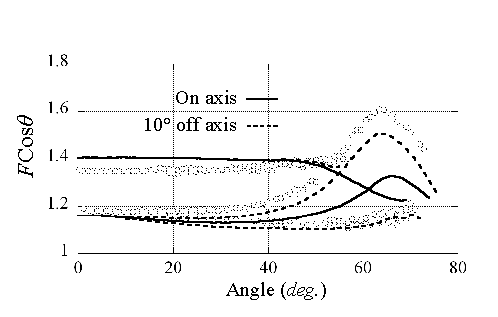
\includegraphics[scale=0.9]{Chapter-dHvABaFe2P2/Figures/AngleDepMeasurements/BaselMisalignment/BaselMisalignment}
        \caption{Portion of the measured \ac{FFT} peaks taken towards the `$[100]$' direction. Superimposed is angle plots calculated from \ac{DFT}. Solid is calculated for the field rotating down to $[100]$, dotted is rotated down to 10\degree off $[100]$ in the basel plane.}
        \label{Fig:ResD:BaselMisalignment}
    \end{center}
\end{figure}
For the $[100]$ direction it became apparent from the fact that the \ac{DFT} and the measured curves were qualitatively different that the field was not perfectly aligned with the $[100]$ axis of the sample. Figure~\ref{Fig:ResD:BaselMisalignment} shows how the measured data (circles) does not align well with the plots calculated for rotations towards $[100]$ (solid) but does align well with plots towards an axis which is rotated \unit{10}{\degree} within the $ab$-plane from the $[100]$ direction. A \unit{10}{\degree} misalignment is within the estimated basel alignment error for the microscope images. The data will continue to be labelled as in the $[100]$ plane however for convenience.

In the first place, these shifts were applied as they conveniently and effectively corrected the Fermi surface energies, however the question arises as to whether there is any physical significance to be attached to them. The technique of rigid energy corrections has been applied to previous measurements on LaFePO\cite{Carrington2009} and SrFe$_2$P$_2$\cite{Analytis2009} both of which are highly two dimensional systems that exhibit relatively strong nesting characteristics. This is in contrast with measurements on CaFe$_2$P$_2$\cite{Coldea2009} which has a highly three dimensional Fermi surface and no nesting vector. Furthermore the bulbous area of the three dimensional hole surface in \BaFeP which does not nest requires no shifting of the Fermi surface to match \ac{DFT} calculations, whereas the nested neck portion does require a shift. This correlation between nesting and shifts in calculated energy make the spin-density-wave fluctuations that are associated with the nesting phenomena an obvious candidate for the cause of the discrepancy between \ac{DFT} calculation and experiment.


\subsubsection{Shifting the \ac{DFT} calculations proportional to orbital character}
\label{Sec:ResD:ShiftingDFTPropToOrbitalCharacter}

Figure~\ref{Fig:ResD:Band2DCharacter} shows the partial orbital character for for each of the bands along the path of Fermi surface contour in a $[110]$ slice through the \BaFeP \ac{BZ} as a function of $k_z$. The top row of plots show the character broke down by atomic contribution, the middle row is broken down by the $s$, $p$, $d$ and $f$ contributions to the iron contribution and the bottom row breaks down the iron $d$ character into its sub orbitals.
\begin{figure}[htbp]
    \begin{center}
        \includegraphics[scale=0.95]{Chapter-dHvABaFe2P2/Figures/AngleDepMeasurements/BandCharacterVsKz/AllBandCharacterVsKz}
        \caption{Partial characters along the Fermi surface contour in the 110 slice (shown in insets) vs. $k_z$. Top row is the chaacrter broken down by each atom, middle row is the iron contribution broken down into the $l$ orbital contributions, the bottom row is the iron $d$ orbital contributions broken down into its suborbitals.}
        \label{Fig:ResD:Band2DCharacterVsKz}
    \end{center}
\end{figure}
We can see the vast majority of Fermi surface chaarcter is due to the iron atomic contributions with some phosphor for bands 2 and 3 which corresponds well to the notion of FeP conducting planes \TODO{Why does the total not sum to 1?}. For all the bands, the overwhelming majority of the contribution from the iron atoms is from the $d$ orbitals and so other contributions are ignored.

Band $2$ has very little basel-plane \Dxy and \DxTwoyTwo character close to the Fermi level but shows a significant amount of \DzTwo character at the wide region of the Fermi surface and \DxzDyz character at the narrow region. Evidently, energy shifts could be applied which are scaled to either the \DzTwo and \DxzDyz orbital character in order that we obtain a smooth energy shift transition between the narrow and wide regions discussed previously. 

Energy shifts were applied across the full three dimensional \ac{BZ} for band $2$ using the following two scalings which were determined by trial and error fitting of the data,
%%
\begin{align*}
\textrm{\DzTwo:}\quad \Delta\epsilon &= 0.002 - 0.0052 \left[1 - \frac{\epsilon - 0.033}{0.2205 - 0.033}\right] \\
\textrm{\DxzDyz:}\quad \Delta\epsilon &= 0.002 - 0.0052 \left[\frac{\epsilon - 0.0946}{0.3135 - 0.0946}\right]
\end{align*}
%%
Note that these scalings ensure that the energy shift applied varies between \unit{-32}{\milli Ry} and \unit{2}{\milli Ry} which are slightly different to the values applied when rigidly shifting the band. This is due to the fact that the Fermi surface area measured in the narrow region is affected more and more by the size of the Fermi surface in the wide region (and vice-versa) as the azimuthal angle gets higher. The calculated area deviates from the measured area which results in the crossing of the calculated rotation plot with the measured rotation plot shown in the first panel of figure~\ref{Fig:ResD:Band2DCharacterRigidComparison}. So when the rigid shifts were being determined, values were chosen which best lines up along the full length of the curve -- one which will be slightly lower than if we were to match the plots exactly at $\theta=0^\circ$.

\begin{figure}[htbp]
    \begin{center}
        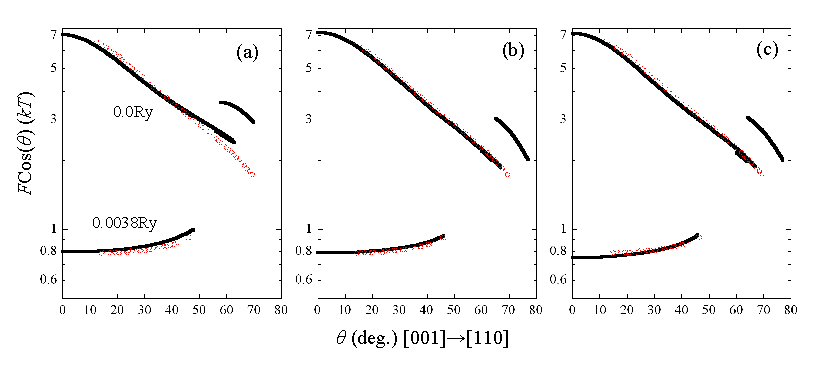
\includegraphics[scale=0.8]{Chapter-dHvABaFe2P2/Figures/AngleDepMeasurements/BandCharacterRotPlot/Band2_110_RotPlot_Comparison}
        \caption{dHvA frequencies for band 2 multiplied by the cosine of the angle of the $H$ field. $H$ field directed along $[001]\rightarrow[110]$. Open circles are measured data, solid lines represent (a) rigidly shifted \ac{DFT} calculations, (b) \ac{DFT} calculations shifted proportional to \DzTwo orbital character, (c) \ac{DFT} calculations shifted proportional to \DxzDyz orbital character.}
        \label{Fig:ResD:Band2DCharacterRigidComparison}
    \end{center}
\end{figure}

The second and third panels of figure~\ref{Fig:ResD:Band2DCharacterRigidComparison} show the rotation plots calculated with the energy shifts applied proportional to \DzTwo and \DxzDyz orbital character respectively. We observe a much better alignment of the measured and calculated data for all angles. Figure~\ref{Fig:ResD:BandCharacterFSShiftComparison} shows the Fermi surfaces before and after shifting using the rigid energy shifts for bands $1$, $3$ and $4$ and using shifts scaled to \DzTwo orbital character for band $2$. Figure~\ref{Fig:ResD:FullBandCharacterFermiSurface} shows the assembled unit cell for \BaFeP from the corrected \ac{DFT} calculations and figure~\ref{Fig:ResD:ShiftedBandStructure} shows the shifted band structure for the bands that cross the Fermi level.
%%
\begin{figure}[htbp]
    \begin{center}
        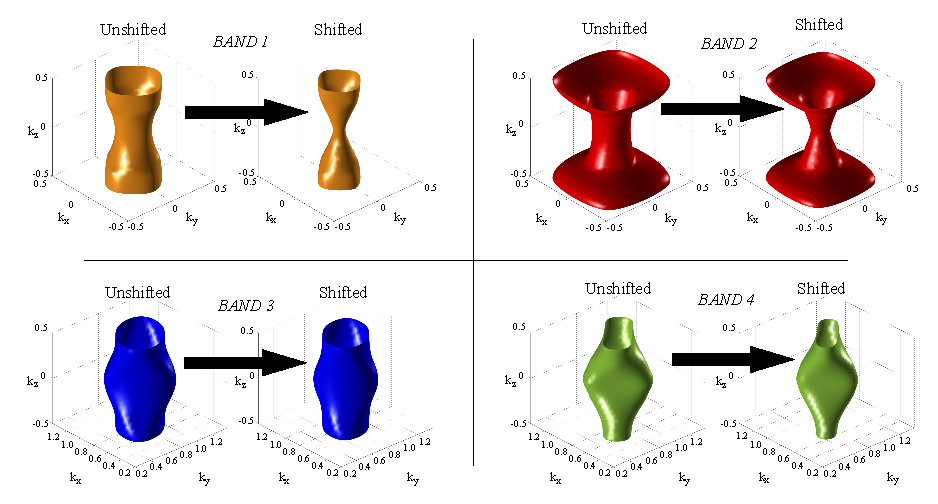
\includegraphics[scale=0.8]{Chapter-dHvABaFe2P2/Figures/AngleDepMeasurements/BandCharacterFermiSurface/BandCharacterFermiSurfaceShiftComparison}
        \caption{Comparison of Fermi surfaces according to \ac{DFT} calculations both before and after shift corrections are applied. Rigid shifts are applied to bands 1, 3, 4 and shifts proportional to \DzTwo character are applied to band 2.}
        \label{Fig:ResD:BandCharacterFSShiftComparison}
    \end{center}
\end{figure}
%%
\begin{figure}[htbp]
    \begin{center}
        \includegraphics[scale=0.7]{Chapter-dHvABaFe2P2/Figures/AngleDepMeasurements/BandCharacterFermiSurface/FullBandCharacterFermiSurface}
        \caption{Fully assembled Fermi surface in the first \ac{BZ} of \BaFeP as determined by \ac{DFT} calculations corrected by either rigid energy shifts (bands 1, 3, 4) or shifts proportional to \DzTwo character (band 2)}
        \label{Fig:ResD:FullBandCharacterFermiSurface}
    \end{center}
\end{figure}
%%

The final corrections show the \ac{DFT} calculations being adjusted in size only for the electron and inner hole surfaces with overall shrinking of volume, the outer hole surface is adjusted in shape as well. Volume calculations as a percentage of the \ac{BZ} are given for each of the Fermi surfaces before and after shifting in table~\ref{Table:ResD:FermiSurfaceVolumes},
\begin{table}
    \begin{center}
           \caption{Volumes of the shifted and unshifted Fermi surfaces as a percentage of \ac{BZ} volume.}
        \begin{tabular}[htbp]{lrrr}
\toprule
Band    & Unshifted    & Shifted \DzTwo    & Shifted \DxzDyz \\
\midrule
1  & 5.54\%    & 2.28\%    & 2.28\%    \\
2  & 10.37\%   & 9.74\%    & 9.64\%    \\
3  & (-)9.58\% & (-)7.89\% & (-)7.89\% \\
4  & (-)6.39\% & (-)4.49\% & (-)4.49\% \\
\midrule
Total & -0.065\%    & -0.352\%  & -0.450\%  \\
\bottomrule
        \label{Table:ResD:FermiSurfaceVolumes}
        \end{tabular}
    \end{center}
\end{table}
The volumes compensate better before the shifts by a small amount ($\sim$\unit{0.4}{\%}) with the shifts proprtional to \DxzDyz being slightly closer to the unshifted volume.

\section{Obtaining the Fermi surface for members of the \BaFePAs series}

We can use existing literature measurements of the Fermi surface at $x=0.38$ from Yoshida \etal \cite{Yoshida2010}, $x=0.63$ from Analytis \etal \cite{Analytis2010c} and a range between $0.4 < x < 1.0$ from Shishido \etal \cite{Shishido2010} to obatain an approximate relation for the size of Fermi surface orbits across the \BaFePAs series. Figure~\ref{Fig:ResD:SeriesRecipe} shows the maximum and minimum orbit sizes with the field along the $c$-axis from these papers along with data presented in this thesis.
\begin{figure}[htbp]
    \begin{center}
        \includegraphics[scale=1.1]{Chapter-dHvABaFe2P2/Figures/AngleDepMeasurements/SeriesRecipe/SeriesRecipe}
        \caption{Left panel shows the trend in electron orbit size at $\theta=0\degree$ over the series, right panel show the hole orbit size trends. Dotted lines show linear fits to the data.}
        \label{Fig:ResD:SeriesRecipe}
    \end{center}
\end{figure}
It may be possible to apply a linear scaling to determine the intermediate orbit sizes however there are a number of assumptions that need to be made. 

Firstly we cannot apply Vegard's law beyond a structural transition in the series meaning we cannot extrapolate to the orthorhombic state at the low $x$ end of the phase diagram. The measurement by Yoshida et al. at $x=0.38$ roughly coincides with the edge of the orthorhombic transition as shown in figure~\ref{Fig:ResD:PhaseDiagram} but was found to be tetragonal and so we can use to to define the lower limit for the extrapolation at low temperatures. There is also a so called `collapsed tetragonal phase' which occurs in the \BaFeAs at a pressure \unit{27}{\giga\pascal}\cite{Mittal2011} at \unit{33}{\kelvin} which could present a problme as we apply chemical pressure. The optimal \Tc of \BaFeAs under pressure is $\sim$\unit{5}{\giga\pascal}~\cite{Colombier2009} and optimal \Tc for the \BaFePAs series is $x\sim0.3$, and so we can very approximately place $x=1$ corresponding to $\sim$\unit{7}{\giga\pascal} which is about half of that required for the collapsed phase transition. Moreover the author is not aware of any reports of the collapsed phase being observed in the \BaFePAs series at atmospheric pressure and so we assume that this is the case. 

There is also the problem of the third hole surface around the $\Gamma$ point which appears in \ac{DFT} calculations. Although it has not been observed in any of the measurements, this is to be expected since electron surfaces generally scatter more and so have a weaker signal to electron pockets and also it may be close in size and shape to other hole surfaces making it difficult to pick out with current \ac{ARPES} resolution.

Looking at figure~\ref{Fig:ResD:SeriesRecipe} we see some inconsistencies which may also throw some doubt onto such a linear fit. Key points from Yoshida \etal are measured from \ac{ARPES} and not \ac{dHvA}. As they were measured at \unit{10}{\kelvin}, this means that the Fermi surface is measured in the superconducting state and not the field suppressed normal state which is the case for the \ac{dHvA} data. It is not clear if this results in different Fermi surfaces. It also should be noted that a linear extrapolation of $\delta$ suggests that it will become more three dimentional as it goes below $x=0.38$, however this does not appear to be supported by the \ac{DFT} results which show it remaining quasi-two dimensional. 

With the above (many) caveats in mind, we can determine a series of linear laws which would approxmately determine the orbit sizes for $0.38 < x < 1.0$ by applying fits to the data in figure~\ref{Fig:ResD:SeriesRecipe}. The results of these fits are given in table~\ref{Table:ResD:SeriesRecipeFits}.
\begin{table}
    \begin{center}
           \caption{Linear relations to determine orbit sizes. Coefficients are of the form $F=mx+c$.}
        \begin{tabular}[htbp]{lrr}
\toprule
Orbit   & $m$   & $c$   \\
\midrule
$\delta_{\textrm{max}}$ & 0.081 & 1.169 \\
$\delta_{\textrm{min}}$ & -1.766 & 1.841 \\
$\gamma_{\textrm{max}}$ & 4.339 & 3.111 \\
$\gamma_{\textrm{min}}$ & 0.698 &  0.071 \\
$\beta_{\textrm{min}}$ & 0.749 & 1.352 \\
$\beta_{\textrm{max}}$ & 0.811 & 1.489 \\
$\alpha_{\textrm{max}}$ & 0.495 & 0.646 \\
$\alpha_{\textrm{min}}$ & 0.946 & 0.404 \\
\bottomrule
        \label{Table:ResD:SeriesRecipeFits}
        \end{tabular}
    \end{center}
\end{table}




\section{Harmonic parametrisation of the Fermi surface}
    \label{Sec:ResD:TightBindingFits}

An analytic form for the Fermi surface can be obtained using a harmonic expansion of sin and cosine functions as described by Bergemann et al\cite{Bergemann2000}. Primarily this was done so as to provide a convenient way to reconstruct the Fermi surface without necessitating DFT calculations however the coefficients also bear some relation to the tight binding model hopping integrals. For strongly correlated systems the tight binding model is generally a poor one to use as it entirely ignores electron correlations. Nonetheless the expansion is as described as,
\begin{equation}
\label{Eqn:ResD:HarmonicExpansion}
k_F(\phi, \kappa) = \sum_{\substack{\mu,\nu \geq 0 \\ \mu \textrm{even}}}
    k_{\mu\nu}\cos\nu\kappa 
    \begin{cases}
        \cos{\mu\phi} \hspace{8pt} &(\mu\mod4 = 0) \\
        \sin{\mu\phi} \hspace{8pt} &(\mu\mod4 = 2)
    \end{cases}
\end{equation}
where $k_F$ is the Fermi surface in k-space, $\kappa = ck_z/2$, $c$ is the unit cell height and $\phi$ is the polar angle.

The two dimensional fits were performed using a least square fitting routine using MATLAB on the DFT data shifted as described in the previous section. Residuals are shown in figure~\ref{Fig:ResD:TightBindingResiduals} \TODO{Make plot of tight binding fit residuals}. The number of terms for the fits were increased until the residuals ceased to change appreciably. Fit parameters are presented in table~\ref{Tab:ResD:HarmonicParams}. Due to the skewed nature of the \kz dispersion of the outer hole surface $20$ terms were necessary to obtain a reasonable fit to the corrected DFT data however electron surfaces could be fitted well with $9$ terms and the inner hole surface with $10$ terms. The final analytical function was then used to create a false energy dispersion on a discrete grid of $k$-points. Extremal orbits were then calculated as a check of how well it matches the original data. The results of this are presented in figure~\ref{Fig:ResD:TightBindingFitRotationPlot}. The analytical function deviates from the measured data at higher angles implying that the 
\begin{figure}[htbp]
    \begin{center}
        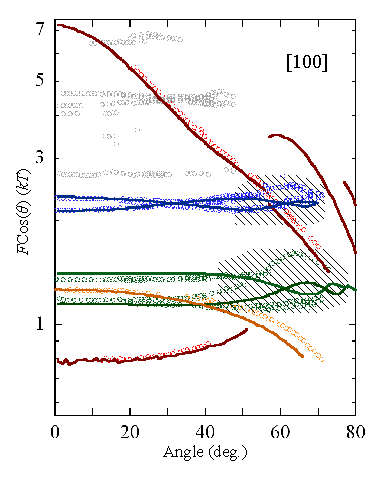
\includegraphics[scale=0.9]{Chapter-dHvABaFe2P2/Figures/AngleDepMeasurements/TightBindingFits/TightBindingFits}
        \caption{Rotation plots for the tight-binding fits calculated from the c-axis down towards $[100]$. As can be seen from the highlighted areas, although the fit residuals are correct to $\sim4\%$, the rotation plot breaks down for high angles in the case of the electron bands.}
        \label{Fig:ResD:TightBindingFitRotationPlot}
    \end{center}
\end{figure}
\begin{table}
    \caption{Harmonic expansion fit parameters performed on the shifted DFT Fermi surfaces}
    \label{Tab:ResD:HarmonicParams}
    \begin{center}
{\small
    \begin{tabular}[htbp]{lrrrr}
\toprule
Factor	& $\alpha$	& $\beta$	& $\gamma$	& $\delta$	\\
\midrule
$k_{00}$	&  1.90796e$^{-1}$	&  2.59538e$^{-1}$	&  2.58282e$^{-1}$	&  1.35031e$^{-1}$	\\
$k_{02}$	& -1.32049e$^{-2}$	& -1.01956e$^{-3}$	&  0		& 0		\\
$k_{04}$	&  9.24279e$^{-4}$	&  4.28603e$^{-4}$	& -1.01085e$^{-2}$	&  1.95065e$^{-3}$	\\
$k_{20}$	&  4.30196e$^{-4}$	& -1.51226e$^{-4}$	& -1.46090e$^{-1}$	& -6.75502e$^{-2}$	\\
$k_{22}$	&  3.23365e$^{-4}$	&  1.91896e$^{-4}$	&  0		& 0		\\
$k_{24}$	& -9.30815e$^{-2}$	& -4.23320e$^{-2}$	&  1.13859e$^{-2}$	& -5.31077e$^{-3}$	\\
$k_{40}$	& -1.64499e$^{-2}$	&  5.02893e$^{-3}$	&  6.15148e$^{-2}$	& -5.70262e$^{-3}$	\\
$k_{42}$	& -1.49159e$^{-2}$	& -7.07858e$^{-3}$	&  0		& 0		\\
$k_{44}$	& -6.14076e$^{-4}$	& -2.86767e$^{-4}$	& -9.49526e$^{-3}$	&  5.28982e$^{-3}$	\\
$k_{60}$	& 0		& 0		& -1.85170e$^{-2}$	& -1.22242e$^{-3}$	\\
$k_{64}$	& 0		& 0		& -9.04247e$^{-4}$	& -2.82851e$^{-4}$	\\
$k_{80}$	& 0		& 0		& -6.79607e$^{-3}$	& -2.22767e$^{-3}$	\\
$k_{84}$	& 0		& 0		&  1.61746e$^{-3}$	& -1.90500e$^{-3}$	\\
$k_{100}$	& 0		& 0		&  1.07007e$^{-2}$	& 0		\\
$k_{104}$	& 0		& 0		&  7.97948e$^{-4}$	& 0		\\
$k_{120}$	& 0		& 0		& -3.89161e$^{-3}$	& 0		\\
$k_{124}$	& 0		& 0		& -1.57292e$^{-3}$	& 0		\\
$k_{140}$	& 0		& 0		& -1.81052e$^{-3}$	& 0		\\
$k_{144}$	& 0		& 0		&  3.81207e$^{-4}$	& 0		\\
$k_{160}$	& 0		& 0		&  3.04268e$^{-3}$	& 0		\\
$k_{164}$	& 0		& 0		&  1.14420e$^{-3}$	& 0		\\
$k_{180}$	& 0		& 0		& -1.07753e$^{-3}$	& 0		\\
$k_{184}$	& 0		& 0		& -4.92181e$^{-4}$	& 0		\\
\bottomrule
    \end{tabular}
}
    \end{center}
\end{table}

% Band 4
% nu_cos_vals = [0 2 4];
% mu_cos_vals = [0 4];
% mu_sin_vals = [2];
% BAND_NUM = 4;
% OUT_FILENAME = 'band4_pseudo_fs.mat';
% P = [0.190795650551417;-0.0132049241203695;0.000924278555081638;0.000430196076110210;0.000323365284403928;-0.0930815369372282;-0.0164499250846804;-0.0149158554339246;-0.000614076088937712];

% Band 3
% nu_cos_vals = [0 2 4];
% mu_cos_vals = [0 4];
% mu_sin_vals = [2];
% BAND_NUM = 3;
% OUT_FILENAME = 'band3_pseudo_fs.mat';
% P = [0.259537885523148;-0.00101956346539010;0.000428602835795347;-0.000151225676919844;0.000191895525922163;-0.0423319597296428;0.00502893573615497;-0.00707857925603053;-0.000286767052816500];

% Band 2
% nu_cos_vals = [0 2 4 6 8 10 12 14 16 18];
% mu_cos_vals = [0 4];
% mu_sin_vals = [];
% BAND_NUM = 2;
% OUT_FILENAME = 'band2_pseudo_fs.mat';
% P = [0.258282295891213;-0.0101085190499327;-0.146089742845922;0.0113858941052011;0.0615148335223954;-0.00949526005728540;-0.0185169711239324;-0.000904247435640945;-0.00679607129328513;0.00161745790960140;0.0107007232759639;0.000797948298873890;-0.00389161131091256;-0.00157292133954998;-0.00180519311058468;0.000381207138913101;0.00304267547098585;0.00114419875689493;-0.00107753360762167;-0.000492181334709838];

% Band 1 
% nu_cos_vals = [0 2 4 6 8];
% mu_cos_vals = [0 4];
% mu_sin_vals = [];
% P = [0.135031574336540;0.00195065231744799;-0.0675502357038337;-0.00531077032608857;-0.00570262272420267;0.00528982052397907;-0.00122242158640231;-0.000282850535526285;-0.00227673928224173;-0.00190499796892254]




\section{Susceptibility calculations}
    \label{Sec:ResD:SubsceptibilityCalculation}

To verify that we do get enhanced susceptibility, which may lead to a spin-density wave state, the $q$-dependant susceptibility -- described in section~\ref{Sec:Theo:Susceptibility} -- was calculated. Since the Lindhard function takes the sum over all energies in the \ac{BZ}, there may be some concern that the rather crude adjustments to the \ac{DFT} calculations performed in the previous section -- which have only been verified to be correct for energies at the Fermi surface -- may give erroneous results. However the nature of the Lindhard function means that far greater weight is given to energies that are near the Fermi surface. Figure~\ref{Fig:ResD:ShiftedBandStructure} shows the `spaghetti plot' with the energies tweaked as described in the previous section. We see that there are discontinuities in band 2, most notably between $Z$ and $\Sigma_1$, due to the correction applied proportional to the \DzTwo{} character, however these are reasonably far from the Fermi level and so should not affect the calculations significantly.
\begin{figure}[htbp]
    \begin{center}
        \includegraphics[scale=0.9]{Chapter-dHvABaFe2P2/Figures/AngleDepMeasurements/ShiftedBandStructure/ShiftedBandStructure}
        \caption{Band structure for the bands that cross the Fermi surface shifted to fit the dHvA data. (a) and (b) give an idea of the granularity of the \WIEN{} calculation at the Fermi surface. Inset shows the path around the \ac{BZ}.}
        \label{Fig:ResD:ShiftedBandStructure}
    \end{center}
\end{figure}

Calculations were performed using the \code{calc_x0.m} code described in section~\ref{Sec:Exp:Susceptibility} using a $93\times93\times93$ grid of energy values that covered the first \ac{BZ}. We will need to smooth over the granularity of the \WIEN{} band model since for the imaginary part at least, the calculation is very sensitive to slight imperfections in cancellation near the Fermi energy. Referring to figure~\ref{Fig:ResD:ShiftedBandStructure}, there are two regions in the marked (a) and (b) which show points around the Fermi level as they are spaced in the $93\times93\times93$ model. (a) is particularly steep and has a $\Delta \epsilon/\Delta\textrm{pt.} = \unit{0.0760}{\electronvolt}$ and (b) is more typical of the gradient at the Fermi level and has $\Delta \epsilon/\Delta\textrm{pt.} = \unit{0.0368}{\electronvolt}$. So the energy scale that will need to compensated is $\sim$\unit{2-5\ten{-3}}{\textrm{\textrm{Ry}}}.

\begin{figure}[htbp]
    \begin{center}
        \includegraphics[scale=0.9]{Chapter-dHvABaFe2P2/Figures/Susceptibility/RangeDeltaOmega/RangeDeltaOmega}
        \caption{Qualitative plots of the real and imaginary part of the Lindhard susceptibility calculated at $k_z=\pi$ for $T=\unit{157}{\kelvin}$ and a range of $\delta$ and $\omega$ values.}
        \label{Fig:ResD:RangeDeltaOmega}
    \end{center}
\end{figure}

Susceptibility was calculated for a wide range of magnitudes of $\delta$ and $\omega$ in order to gauge qualitative behaviour with the resulting plots shown in figure~\ref{Fig:ResD:RangeDeltaOmega}. Both the real and imaginary parts undergo qualitative changes as the parameters are adjusted above the spacing corresponding to the typical gap in energy between points. The imaginary part also undergoes a qualitative change when $\omega$ falls below \unit{1\ten{-5}}{\textrm{Ry}} and there is also an increase in noise when $\delta$ falls below a similar energy threshold. We continue using $\delta=1\ten{-3}$ and $\omega=1\ten{-3}$ which correspond approximately the energy scale of the spacing as well as the energy scale of the temperature smearing.

\begin{figure}[htbp]
    \begin{center}
        \includegraphics[scale=0.9]{Chapter-dHvABaFe2P2/Figures/Susceptibility/2DSusceptibility/2DSusceptibilityPlusAltKz}
        \caption{Real and imaginary part of the Lindhard susceptibility are plotted on the left and right respectively. Upper panels are at $k_z=\pi$ and lower are at $k_z=0$. For these calculations $\delta=1\ten{-3}$, $\omega=1\ten{-3}$ and $T=\unit{157.88}{\kelvin}$. Insets show contour plots for the respective surface plots.}
        \label{Fig:ResD:2DSusceptibility}
    \end{center}
\end{figure}
The upper panel of figure~\ref{Fig:ResD:2DSusceptibility} shows the quantified plots for the real and imaginary parts of the susceptibility at the chosen values of $\delta$ and $\omega$. The contour plots in the insets show the two-fold symmetry due to the choice of $k_z=\pi$. Unlike LaFeAsOF where the two dimensional approximation is a good one, this is not necessarily the case for \BaFeP{} which features a strongly three-dimensional hole band and some warping of the electron bands. The lower panels present the same calculation performed at $k_z=0$ which shows little change other than a rotation of the susceptibility bias due to the screw symmetry of the electron bands.

\begin{figure}[htbp]
    \begin{center}
        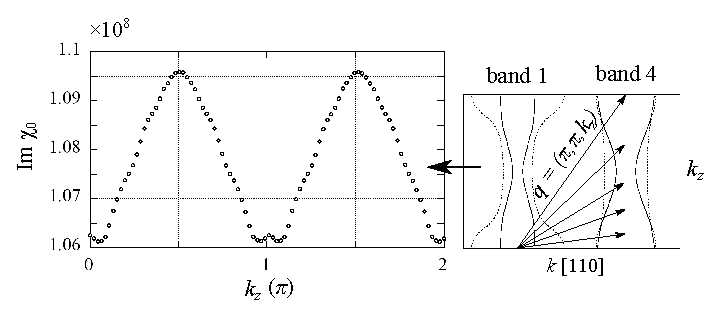
\includegraphics[scale=0.7]{Chapter-dHvABaFe2P2/Figures/Susceptibility/NestingVector/NestingVector}
        \caption{Left panel shows the imaginary part of the Lindhard susceptibility between bands summed with their reciprocals for $q=(\pi, \pi, k_z)$ over the height of the \ac{BZ}. We see enhancements at $k_z=\pi/2,3\pi/2$ for bands 1-4 and 2-3 and at $k_z=0,\pi,2\pi$ for bands 2-3 and 2-4.}
        \label{Fig:ResD:NestingVector}
    \end{center}
\end{figure}
To verify that there is indeed a nesting conditions at some $k_z$ for $q=(\pi, \pi, k_z)$ figure~\ref{Fig:ResD:NestingVector} presents the imaginary part of the susceptibility vs. $k_z$ for a range of nesting vectors. Each coupling of bands is summed both ways --- e.g. 4-1 is summed with 1-4 --- and plotted in order to obtain the residual difference due to $\omega$. Unsurprisingly, we see that self coupling results in very little weight with hole-hole and electron-electron coupling also resulting in little weight. The strongest component is due to bands 2-4 which also demonstrates a strong enhancement of around $25\%$ at $k_z=0,\pi,2\pi$. Band 2 also couples strongly with band three at the same $q$ vectors with around a $17\%$ enhancement. Band 1 couples strongly with band 4 but at $k_z=\pi/2,3\pi/2$ with the largest enhancement of around $38\%$. Band 1 also couples less strongly with band $3$ at the same $k_z$ with an enhancement of around $15\%$. The total susceptibility is determined mostly by the coupling of band 2 but only has a relatively moderate enhancement of around $7.4\%$ at $k_z=0,\pi,2\pi$.

Figure~\ref{Fig:ResD:ZSlices} shows cross sections of the final corrected Fermi surfaces showing the basal-plane at the bottom of the unit cell ($k_z=0$), quarter of the way up, ($k_z=0.25$) and halfway up ($k_z=0.5$). The inner hole surface (band 1) at $k_z=0.5$ directly matches the size and shape of the inner electron surface (band 4) at $k_z=0.25$ which is the likely cause of the strong enhancement observed in the susceptibility. Moreover, the bands share similar predominant \DxzDyz{} orbital character. The strong enhancements between bands 2 and 4 are also shown in the figure as a dashed arrow.

\begin{figure}[htbp]
    \begin{center}
        \includegraphics[scale=0.9]{Chapter-dHvABaFe2P2/Figures/AngleDepMeasurements/ZSlices/ZSlices}
        \caption{Cross sections of the corrected Fermi surface in the $ab$ plane (panels 1, 2 and 3) and in the $[110]$ plane (panel 4). Markings correspond to the orbital character of the Fermi surface slices. Two nesting vectors are shown as long arrows.}
        \label{Fig:ResD:ZSlices}
    \end{center}
\end{figure}

These enhancements at $q=(\pi, \pi)$ show that partial nesting does indeed occur in this material demonstrating that this condition alone is not sufficient for superconductivity to occur. This concludes the Fermiology results, we now move onto the mass enhancements.




\section{Determining the spin mass}

Following the method in section~\ref{Sec:Exp:MeasuringSpinMass} we begin by taking a variety of spin masses using the cylindrical approximation. Figure~\ref{Fig:ResD:Band4SpinMassCylindrical} shows \ac{FFT} amplitudes for a portion of the $\alpha$ electron pocket taken over a range of angles towards the $[100]$ direction. The shaded areas are bound to the areas where we believe the amplitudes go to zero as defined by the overall shape of the curve and the splitting of the peaks. The upper panel shows the particular oscillation that most closely matches the zeros in the data as well as its upper and lower bounds to quantify the possible error. The lower panel shows the next and previous set of oscillations in order to demonstrate that the selected oscillation in the top panel is indeed the best fit. In the cylindrical case the best fit is given by \TODO{XXXXX} with an error of \TODO{XXXX}.
\begin{figure}[htbp]
    \begin{center}
        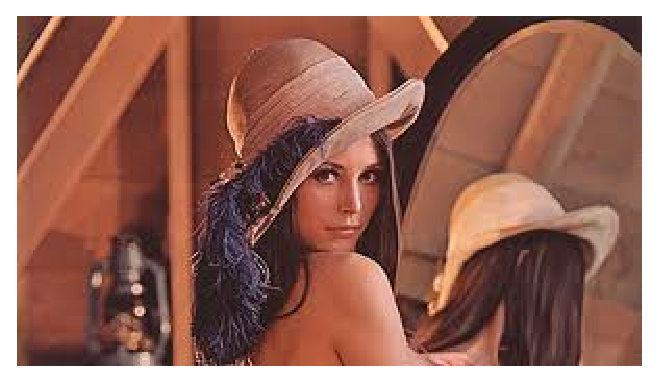
\includegraphics[scale=0.9]{Misc/TODO}
        \caption{Measured amplitude of \ac{FFT} peaks across a range of angles for the portion of data shown in the inset. Curves corresponding to the $A_S$ term calculated using the cylindrical apporximation are superimposed. Upper panel shows the best fitting data and its bounds, the lower portion shows fitting to the next oscillation along which clearly demonstrates the misalignment. Shaded areas are zones where we believe the spin zeros are located in the data.}
        \label{Fig:ResD:Band4SpinMassCylindrical}
    \end{center}
\end{figure}
We now contrast this with a spin mass determination using a band mass calculated from \ac{DFT}. Figure~\ref{Fig:ResD:DFTBandMassBand4} shows the band mass as calculated from the shifted \ac{DFT} energies for band 4. On the plot is an order 8 polynomial fit as well as the corresponding cylindrical approximation curve for comparison.
\begin{figure}[htbp]
    \begin{center}
        \includegraphics[scale=0.9]{Chapter-dHvABaFe2P2/Figures/Mass/DFTBandMassBand4/DFTBandMassBand4}
        \caption{Band masses calculated from \ac{DFT} of band 4 taken over a range of angles rotating towards the $[100]$ direction. A fit to and order 8 polynomial is shows as well as a comparitive fit suing the cylindrical approximation.}
        \label{Fig:ResD:DFTBandMassBand4}
    \end{center}
\end{figure}
Taking the polynomial from the fit to the \ac{DFT} band mass calulcations as the band mass for the inspection of the $A_S$ term, figure~\ref{Fig:ResD:SpinMassFromDFTBand4} shows the revised best fit. Now the fit values gives a spin mass of \TODO{XXXX} with an error pf \TODO{XXXX}.
\begin{figure}[htbp]
    \begin{center}
        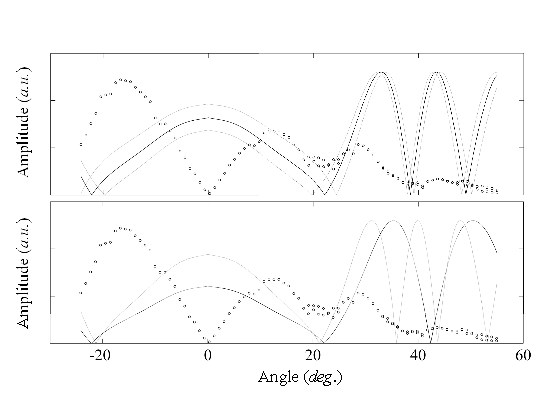
\includegraphics[scale=0.8]{Chapter-dHvABaFe2P2/Figures/Mass/SpinMassBand4/SpinMassBand4}
        \caption{Measured amplitude of \ac{FFT} peaks across a range of angles for the portion of data shown in the inset.  Curves corresponding to the $A_S$ term calculated using the cylindrical apporximation are superimposed. Upper panel shows the best fitting data and its bounds, the lower portion shows fitting to the next oscillation along which clearly demonstrates the misalignment. Shaded areas are zones where we believe the spin zeros are located in the data.}
        \label{Fig:ResD:SpinMassFromDFTBand4}
    \end{center}
\end{figure}
Given that a more accurate fit is obtained by using the \ac{DFT} calculated band masses, table~\ref{Table:ResD:SpinMassValues} shows more spin mass values calculated using this technique with the full graphs given in Appendix~\ref{Appendix:SpinMassPlots}.
\begin{table}
    \begin{center}
           \caption{Spin mass values calculated using inspection of measured data. Values calculated from \ac{DFT} were used for the band mass term.}
        \begin{tabular}[htbp]{ll}
\toprule
Band    &   $m^*_S$ \\
\midrule
\TODO{XXXX} & \TODO{XXXX} \\
\bottomrule
        \label{Table:ResD:SpinMassValues}
        \end{tabular}
    \end{center}
\end{table}



\section{Determining the thermal effective mass}


\subsubsection{Basic \ac{LK} formula fitting}

A series of field sweeps were taken with $H$ at \unit[12]{\degree}, \unit[28]{\degree} and \unit[46]{\degree} from $[001]$ in the $[110]$ direction. These were performed at a variety of temperatures from base ($\approx\unit[0.3]{K}$) to above \unit[2]{K}. Corrections were applied as detailed in section\ref{Sec:Exp:TemperatureCorrection}. \Fig~\ref{Fig:ResD:SimpleLKFits} shows the Fourier amplitude of various peaks as a function of temperature along with fits to equation~\ref{Eqn:Exp:TempTermOscillationAmp}. The field range for the FFT was was necessarily large enough that individual peaks did not overlap and also could be observed across a reasonable range of temperatures but also small enough so that the $B$ dependent Dingle factor did not play too large a role and so an average $B$ field can be assumed. The results from these fits are shown in table \ref{Tab:ResD:EffectiveMassResults} along with the fit ranges. All FFTs in the plot were taken over an interval of \unit[12--18]{T} with the exception of the $\gamma_2$ fit which was taken between \unit[16-18]{T} so as to attain an appreciable peak. The standard deviation as calculated by randomly varying the temperature values by the estimated error (\unit[0.06]{K}) 1000 times and then taking the standard deviation of the fitted $m^*$ values.
\begin{figure}[htbp]
    \begin{center}
        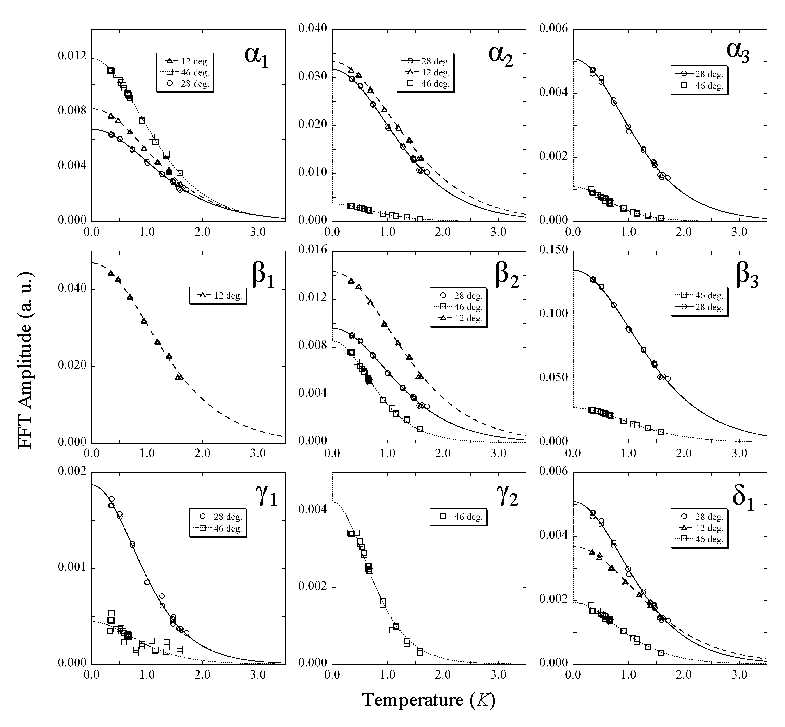
\includegraphics[scale=0.9]{Chapter-dHvABaFe2P2/Figures/Mass/SimpleLKFits/SimpleLKFits}
        \caption{Fits to the temperature dependant part of the \LK formula. }
        \label{Fig:ResD:SimpleLKFits}
    \end{center}
\end{figure}
Table \ref{Tab:ResD:EffectiveMassResults} also shows gives a result, marked with a dagger, taken with a different field range. These fits give quite different values for the effective mass, indicating that the average field approximation is not a valid one.

\subsubsection{Retrofitting ansatz LK formulae}

The measurements presented in the previous section were further refined using the the ansatz LK formulae as described in section~\ref{Sec:Exp:LKRetrofitting}. \Fig~\ref{Fig:ResD:DingleTermExtractionFits} shows some sample fits used to extract the Dingle terms used in the ansatz fit functions.
\begin{figure}[htbp]
    \begin{center}
        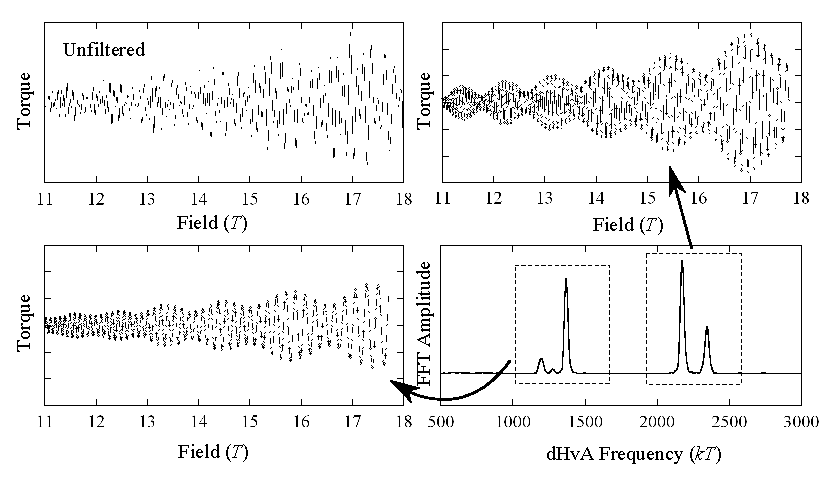
\includegraphics[scale=0.9]{Chapter-dHvABaFe2P2/Figures/Mass/FittingDingleTerm/FittingDingleTerm}
        \caption{Top left panel shows torque data for data taken at \unit[12]{\degree} towards the $[110]$ direction at \unit[0.35]{K} with a polynomial background subtracted. Bottom right shows the FFT and the two filter windows to produce the filtered torque plots in the top right and bottom left. Filtered plots are fitted to extract the Dingle term for each frequency.}
        \label{Fig:ResD:DingleTermExtractionFits}
    \end{center}
\end{figure}
Table\ref{Tab:ResD:EffectiveMassResults} lists the extracted Dingle terms for each peak of the Fermi surface and the subsequent results of the retrofitted calculations for the effective masses. The various field limits were chosen in order to either obtain a clearly delimited peak in the lower field cases or to obtain a signal from a weak peak in the higher field cases.


\subsubsection{`Microfitting' the LK formula}

A second attempt at refining the LK fits was performed by applying the microfit technique desribed in section~\ref{Sec:Exp:LKMicrofitting}. $1.5$ oscillations were fit at a time Filtering the data beforehand is not always straightforward due to close proximity of neighbouring peaks. The stronger peaks from the $\alpha$ and $\beta$ Fermi surfaces show banding of the masses and a clear trending of the results to one of a few values which have been highlighted in yellow. Data in these regions were averaged to give the values in table \ref{Tab:ResD:EffectiveMassResults}.

All filtered using function $\textit{F}_{\textrm{filt}}(x) = \textit{F}(x) \times 1/2 [\tanh{(\pi(x - x_{\textrm{low}})/w)} + \tanh{(-\pi(x - x_{\textrm{high}})/w})]$ where $\textit{F}$ is the Fourier transform of the torque data, $x$ is the dHvA frequency, $x_{\textrm{low}}$ and $x_{\textrm{high}}$ are the lower and upper limits of the filter range respectively and $w$ determines the trail off slope of the filter function. For all measurements $w=10$.
%%
\begin{figure}[htbp]
    \begin{center}
        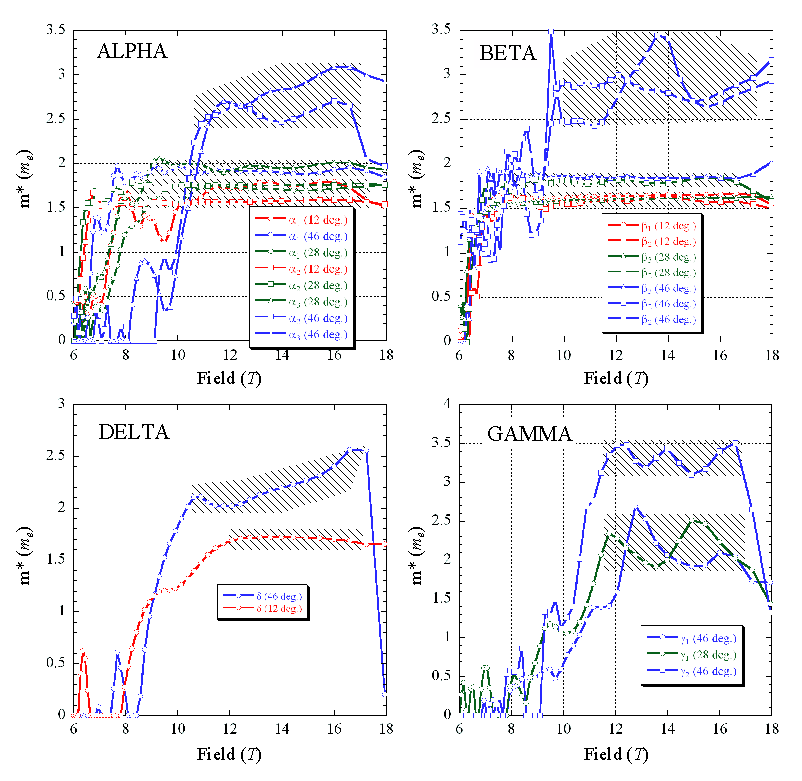
\includegraphics[scale=0.7]{Chapter-dHvABaFe2P2/Figures/Mass/MicroFits/MicroFits}
        \caption{Effective temperature dependant masses extracted from fits to between one and three dHvA oscillations in the measured data. See Appendix\ref{Appendix:MicroFitParams} for a full list of parameters for each set of fits.}
        \label{Fig:ResD:MicroFits}
    \end{center}
\end{figure}
%%
\begin{sidewaystable}
    \begin{center}
        \caption{Comparison of the three effective mass calculation techniques. First grey band shows the plain \LK fitted results, following white band details the retrofitted effective mass calculations, following grey band details the microfitted results, and the final band details the band masses from DFT calculations and the three results normalised to these band masses. Result marked with a dagger is repeated with a different field range. Entries marked `NA' had a signal too weak to extract an $\alpha$ value and so microfitting was not possible.}
{\small
        \begin{tabular}[htbp]{rrlrrrrrrrrrrrr}
\toprule
Angle	& Freq.	& Label	& $m^*_{\textrm{LK}}$	& $m^*_{\textrm{ret.}}$	& $\alpha$	& $B_{\textrm{min.}}$	& $m^*_{\textrm{mic.}}$	& $B_{\textrm{max.}}$	& $B_{\textrm{min.}}$	& Filt. Width	& $m^*_{\textrm{b}}$	& $\frac{m^*_{\textrm{LK}}}{m^*_{\textrm{b}}}$	& $\frac{m^*_{\textrm{ret.}}}{m^*_{\textrm{b}}}$	& $\frac{m^*_{\textrm{mic.}}}{m^*_{\textrm{b}}}$ \\
\midrule
12	& 1210	& $\alpha_1$	& \cellcolor[gray]{0.9} 1.49(2)$^\dagger$	& 1.69	& 58.68	& 8	& \cellcolor[gray]{0.9} NA	& \cellcolor[gray]{0.9} NA	& \cellcolor[gray]{0.9} NA	& \cellcolor[gray]{0.9} NA	& 1.04	& 1.43	& 1.63	& NA \\
12	& 1210	& $\alpha_1$	& \cellcolor[gray]{0.9} 1.71(3)	& 1.75	& 58.68	& 12	& \cellcolor[gray]{0.9} 1.75(3)	& \cellcolor[gray]{0.9} 17.0	& \cellcolor[gray]{0.9} 11.0	& \cellcolor[gray]{0.9} 1100--1240	& 1.04	& 1.64	& 1.68	& 1.68 \\
28	& 1269	& $\alpha_1$	& \cellcolor[gray]{0.9} 1.64(2)	& 1.68	& 59.60	& 12	& \cellcolor[gray]{0.9} 1.72(2)	& \cellcolor[gray]{0.9} 17.0	& \cellcolor[gray]{0.9} 11.0	& \cellcolor[gray]{0.9} 1200--1310	& 0.90	& 1.83	& 1.88	& 1.92 \\
46	& 1532	& $\alpha_1$	& \cellcolor[gray]{0.9} 1.86(3)	& 1.90	& 48.79	& 12	& \cellcolor[gray]{0.9} 1.92(2)	& \cellcolor[gray]{0.9} 17.0	& \cellcolor[gray]{0.9} 9.0	& \cellcolor[gray]{0.9} 1430--1585	& 1.00	& 1.86	& 1.90	& 1.92 \\
12	& 1372	& $\alpha_2$	& \cellcolor[gray]{0.9} 1.54(2)	& 1.58	& 45.99	& 12	& \cellcolor[gray]{0.9} 1.57(1)	& \cellcolor[gray]{0.9} 17.0	& \cellcolor[gray]{0.9} 8.0	& \cellcolor[gray]{0.9} 1320--1440	& 0.84	& 1.83	& 1.88	& 1.86 \\
28	& 1530	& $\alpha_2$	& \cellcolor[gray]{0.9} 1.69(2)	& 1.74	& 72.35	& 12	& \cellcolor[gray]{0.9} 1.75(2)	& \cellcolor[gray]{0.9} 17.0	& \cellcolor[gray]{0.9} 8.0	& \cellcolor[gray]{0.9} 1450--1650	& 0.93	& 1.81	& 1.87	& 1.88 \\
46	& 2017	& $\alpha_2$	& \cellcolor[gray]{0.9} 2.49(5)	& 2.56	& 61.06	& 12	& \cellcolor[gray]{0.9} 2.55(11)	& \cellcolor[gray]{0.9} 16.8	& \cellcolor[gray]{0.9} 10.5	& \cellcolor[gray]{0.9} 1970--2100	& 1.83	& 1.36	& 1.40	& 1.40 \\
28	& 1365	& $\alpha_3$	& \cellcolor[gray]{0.9} 1.85(3)	& 1.93	& 115.49	& 12	& \cellcolor[gray]{0.9} 1.97(3)	& \cellcolor[gray]{0.9} 17.0	& \cellcolor[gray]{0.9} 9.5	& \cellcolor[gray]{0.9} 1320--1440	& 1.18	& 1.56	& 1.63	& 1.67 \\
46	& 1930	& $\alpha_3$	& \cellcolor[gray]{0.9} 2.87(7)	& 3.04	& 149.39	& 12	& \cellcolor[gray]{0.9} 2.75(24)	& \cellcolor[gray]{0.9} 17.0	& \cellcolor[gray]{0.9} 10.7	& \cellcolor[gray]{0.9} 1890--1970	& 1.00	& 2.87	& 3.04	& 2.75 \\
12	& 2180	& $\beta_1$	& \cellcolor[gray]{0.9} 1.61(2)	& 1.65	& 51.12	& 12	& \cellcolor[gray]{0.9} 1.63(2)	& \cellcolor[gray]{0.9} 17.0	& \cellcolor[gray]{0.9} 8.0	& \cellcolor[gray]{0.9} 2100--2270	& 0.98	& 1.64	& 1.68	& 1.66 \\
12	& 2350	& $\beta_2$	& \cellcolor[gray]{0.9} 1.56(3)	& 1.62	& 102.36	& 12	& \cellcolor[gray]{0.9} 1.57(3)	& \cellcolor[gray]{0.9} 17.0	& \cellcolor[gray]{0.9} 9.0	& \cellcolor[gray]{0.9} 2270--2450	& 0.86	& 1.81	& 1.88	& 1.82 \\
28	& 2605	& $\beta_2$	& \cellcolor[gray]{0.9} 1.30(2)	& 1.87	& 102.36	& 6	& \cellcolor[gray]{0.9} 1.81(2)	& \cellcolor[gray]{0.9} 17.0	& \cellcolor[gray]{0.9} 8.5	& \cellcolor[gray]{0.9} 2555--2670	& 1.03	& 1.68	& 1.71	& 1.76 \\
46	& 3347	& $\beta_2$	& \cellcolor[gray]{0.9} 1.73(2)	& 1.76	& 34.08	& 12	& \cellcolor[gray]{0.9} 2.86(8)	& \cellcolor[gray]{0.9} 17.3	& \cellcolor[gray]{0.9} 10.0	& \cellcolor[gray]{0.9} 3250--3370	& 1.80	& 1.44	& 1.50	& 1.59 \\
46	& 3381	& $\beta_2$	& \cellcolor[gray]{0.9} 2.59(6)	& 2.69	& 94.57	& 12	& \cellcolor[gray]{0.9} 2.78(32)	& \cellcolor[gray]{0.9} 17.3	& \cellcolor[gray]{0.9} 10.0	& \cellcolor[gray]{0.9} 3365--2500	& 1.80	& 0.88	& 0.90	& 1.55 \\
28	& 2475	& $\beta_3$	& \cellcolor[gray]{0.9} 1.58(2)	& 1.61	& 48.81	& 12	& \cellcolor[gray]{0.9} 1.59(2)	& \cellcolor[gray]{0.9} 17.0	& \cellcolor[gray]{0.9} 8.0	& \cellcolor[gray]{0.9} 2400--2560	& 0.93	& 1.95	& 2.00	& 1.71 \\
46	& 2970	& $\beta_3$	& \cellcolor[gray]{0.9} 1.82(3)	& 1.86	& 40.03	& 12	& \cellcolor[gray]{0.9} 1.86(1)	& \cellcolor[gray]{0.9} 17.0	& \cellcolor[gray]{0.9} 8.5	& \cellcolor[gray]{0.9} 2850--3100	& 1.03	& 2.07	& 2.15	& 1.80 \\
28	& 912	& $\gamma_1$	& \cellcolor[gray]{0.9} 2.13(5)	& 2.22	& 104.38	& 12	& \cellcolor[gray]{0.9} 2.17(18)	& \cellcolor[gray]{0.9} 16.8	& \cellcolor[gray]{0.9} 11.3	& \cellcolor[gray]{0.9} 850--970	& -1.49	& -1.03	& -1.10	& -1.46 \\
46	& 1320	& $\gamma_1$	& \cellcolor[gray]{0.9} 2.19(3)	& 2.30	& 129.82	& 12	& \cellcolor[gray]{0.9} 2.00(37)	& \cellcolor[gray]{0.9} 16.8	& \cellcolor[gray]{0.9} 11.3	& \cellcolor[gray]{0.9} 1270--1370	& -2.04	& -0.91	& -0.95	& -0.98 \\
46	& 4497	& $\gamma_2$	& \cellcolor[gray]{0.9} 3.31(8)	& 3.32	& 91.06	& 16	& \cellcolor[gray]{0.9} 3.31(13)	& \cellcolor[gray]{0.9} 16.8	& \cellcolor[gray]{0.9} 12.2	& \cellcolor[gray]{0.9} 4400--4600	& -1.89	& -1.17	& -1.23	& -1.75 \\
12	& 1270	& $\delta$	& \cellcolor[gray]{0.9} 1.54(2)	& 1.64	& 173.00	& 12	& \cellcolor[gray]{0.9} 1.71(1)	& \cellcolor[gray]{0.9} 17.0	& \cellcolor[gray]{0.9} 12.0	& \cellcolor[gray]{0.9} 1250--1310	& -0.91	& -2.41	& -2.53	& -1.88 \\
28	& 1370	& $\delta$	& \cellcolor[gray]{0.9} 1.85(3)	& 1.93	& 115.49	& 12	& \cellcolor[gray]{0.9} NA	& \cellcolor[gray]{0.9} NA	& \cellcolor[gray]{0.9} NA	& \cellcolor[gray]{0.9} NA	& -0.98	& -1.89	& -1.97	& NA \\
46	& 1626	& $\delta$	& \cellcolor[gray]{0.9} 2.22(4)	& 2.33	& 126.02	& 12	& \cellcolor[gray]{0.9} 2.17(15)	& \cellcolor[gray]{0.9} 17.0	& \cellcolor[gray]{0.9} 10.5	& \cellcolor[gray]{0.9} 1590--1690	& -1.10	& -3.00	& -3.01	& -1.96 \\

\bottomrule
        \end{tabular}
}
        \label{Tab:ResD:EffectiveMassResults}
    \end{center}
\end{sidewaystable}



\section{Conslusions}

The \BaFeP crystal and the subsequent angle dependent \ac{dHvA} measurements are of very good quality as evidenced by a number of traits including the presence of second and third harmonics in the \acp{FFT}, the hole orbits showing up over a wide angular range, the early onset of oscillations at \unit{6}{\tesla} and the observation of the Zeeman splitting of the \ac{FFT} peaks. The crystal appears to be a very clean single crystal although there is some evidence of some misaligned domains, for example from some of the Bragg spots doubling up in the \ac{XRD} and multiple peaks observed in the \ac{FFT} at particular angles -- see for example $\alpha$ towards the $[100]$ direction above $\sim 20\degree$ in figure~\ref{Fig:ResD:AngleSweepMeasured}. There are approximately half a dozen separate peaks observed at this location which implies a similar amount of misaligned domain orientations. This misalignment however does not appear to affect the overall data which largely does not resolve the extra domains.

The Fermiology is largely solved by the angle plots with only a few minor ambiguities.  The $F\cos \theta$ angle dependent plots clearly show approximately level curves for the two hole Fermi surfaces demonstrating that $\alpha$ and $\beta$ are approximately two-dimensional. The hole surface, $\gamma$, deviates at high angles and $\delta$ is strongly three dimensional. Although we cannot say for certain whether $\gamma$ is pinched off or not, based on the rigidly shifted \ac{DFT} we expect that the minima to be small but not zero and was not observed due to low frequency noise in the oscillations.

Previous \ac{dHvA} measurements on BaFe$_2$(As$_{0.37}$P$_{0.63}$)$_2$ by Analytis \etal shown in figure~\ref{Fig:ResD:IdentifyingBands} identified the branch of the \ac{dHvA} angle data at around \unit{500}{\tesla} as the neck of the 2D hole pocket. In our own analysis, it made much more sense to attribute this curve to the neck portion of the 3D hole band, with the neck of the 2D pocket being buried in the low frequency noise. These two different statements are not necessarily incompatible. Since the \ac{DFT} data for the entire series suggests that whilst the 2D hole pocket retains the same shape along the \BaFePAs series, the 3D hole pocket narrows considerably at the $\Gamma$ point and switches from being concentric with the 2D pocket at $x=1$ to crossing through the 2D pocket as $x$ is reduced. However when the spin-orbit interaction is considered in the \ac{DFT} calculations, the crossing of the surfaces causes the bands to be redifined such that the bands do not actually cross, in which case there would not be a Yamaji point as specified in the Analytis paper since the similarly sized orbits at \unit{50}{\degree} angle are not from the same band. An attempt was made to see if there was an enhacement of the oscillation amplitude at the correpsonding putative Yamaji point in the \BaFeP data but the close proximity of the strong oscillations from the electron pockets made this intractable with this particular data set.

Although the Fermi surface appears to nest at the $q=(\pi, \pi, \pi/4)$ as shown in figure~\ref{Fig:ExpD:ZSlices}, the correpsonding imaginary part of the susceptibility data shows stronger enchancements at the $q=(\pi, \pi, \pi/2)$ vector, primarily due to the nesting between the 3D hole fermi surface and the inner electron surface. However the susceptibility calculations do not take into account the orbital character of electrons at these nesting vectors. The dominant character at $q=(\pi, \pi, \pi/2)$ is between regions of \DxzDyz on the narrow portion of the 3D surface and regions that switch between \Dxy and \DxzDyz on the electron surface. This will supress the scattering between the two due to considerations of angular momentum. Notheless the susceptibility shows there are significant enhancements of the imaginary part of the susceptibility repsonse between the electron and hole surfaces and the partial nesting conditions required for spin fluctuations are satisfied. Given that that the system becomes more two dimensional as we approach the superconducting region, this suggests that the nesting is enhanced and the fluctuations become stronger.

Like previous measurements of band structure by \ac{dHvA} in the \BaFePAs materials, the Fermi surfaces are smaller than predicted by \ac{DFT} calculations\cite{Shishido2010, Analytis2010c}. Ortenzi \etal~\cite{Ortenzi2009} posits an explanation based on interband scattering which leads to shrinking of the electron and hole pockets and an enhancement of the effective mass based on relaxing an assumption on the chemical potential being far\footnote{i.e. greater than the scattering boson energy scale} from the electron/hole band edges. Similar moderate effective mass enhacements to what we found in \BaFeP of around $1.4m_e$ were calculated --- albeit modeled on a more two dimensional pnictide, LaFePO --- along with the fact that the theory predicts stronger shifts where interband coupling occurs is supported by the \BaFeP data. The nested portions of the 3D $\delta$ hole band, for example, is strongly shifted where it nests with the electron band but the bulge which does not nest with anything is nto shifted at all. Similar shifts between the measured data and calculations were observed for the sister 122 compound SrFe$_2$P$_2$\cite{Analytis2009} which is also a partially nested material and yet shifts are notably absent for the non-nested 122 pnictide compound CaFe$_2$P$_2$~\cite{Coldea2009} which matched the \ac{DFT} calculations with no ajdustments to the energies. 

% Ortenzi's paper is not specific as to the type of scattering other than it is mediated via a bosonic mode with the prime candidates being \ac{SDW}, \ac{CDW} and phonons. \TODO{More here}

It is not clear at this stage whether the shifting of the Fermi surface proprtional to the electron character for the 3D hole $\delta$ band performed in section~\ref{Sec:ResD:ShiftingDFTPropToOrbitalCharacter} represents anything physical or is simply a convenient and reproducable way to obtain the correct band topology. Settling this question will require further investigation. However it is interesting to note that the energy shifts for the 3D hole surface are proprtional to the \DzTwo and \DxzDyz characters, suggesting there may be a link between the $k_z$ scattering component and energy enhancements. Recalling that the 3D hole surface is where we expect to see the the strongest nesting component this also suggest that the scattering between layers may play a part in supressing superconductivity.

The wide bulge in the 3D hole surface ensures that several terms are needed for the harmonic fits represented in section~\ref{Sec:ResD:TightBindingFits}. For this reason, the harmonic fits simply represent a convenient way to obtain the Fermi surface topology in the case of the 3D hole pocket.


%\clearpage
